% Quick start guide
\documentclass{beamer}

\usetheme {default}

\setbeamertemplate{navigation symbols}{}

% Title page details
\title{Build the World}
\subtitle{with Terraform}
\author{Tim Olson}
\date{\today}

\begin{document}

\begin{frame}
\titlepage
\end{frame}

% ....

\begin{frame}{Outline}

\begin{itemize}
    \item History of Terraform
    \item What exactly is Terraform
    \item Comparing Terraform to other Tools
    \item Components of Terraform
    \item Phases of Terraform
    \item Demos!
\end{itemize}

\end{frame}

% ....

\begin{frame}{History of Terraform}{Let's take a journey to the 2010s}
\begin{itemize}
    \item We have a few newish cloud hosting solutions
    \item AWS, GCP, Azure
    \item For better or worse, in the cloud we have to solve problems in a new way
\end{itemize}

\begin{columns}
    \begin{column}{0.1\textwidth}
        
\includegraphics[width=80px,keepaspectratio]{./assets/aws.png}
    \end{column}
    \begin{column}{0.1\textwidth}
        
\includegraphics[width=80px,keepaspectratio]{./assets/gcp.png}
    \end{column}
    \begin{column}{0.1\textwidth}
        
\includegraphics[width=80px,keepaspectratio]{./assets/azure.png}
    \end{column}
\end{columns}

\end{frame}

% ....

\begin{frame}{Consider the case of an AWS shop}

\begin{itemize}
    \item I'm not managing iptables, I'm using AWS Security Groups
    \item I'm not racking servers, I'm launching EC2 Instances
    \item I'm not configuring Unbound, I'm creating Route53 records
    \item You get the idea... 
\end{itemize}

\vspace{0.3cm}
We're changing where the problem space from configuration management to state management.

\end{frame}

% ....

\begin{frame}{Consider the case of an AWS shop (cont)}

Some problems along our journey:
\vspace{0.3cm}

\begin{itemize}
    \item Is the cloud choice even the right one?
    \item How are you going to create these resources?
    \begin{itemize}
        \item ClickOps - Not reproducible
        \item AWS CLI - A bit cumbersome
        \item Python libraries - Highly complex
    \end{itemize}
\end{itemize}

\vspace{0.3cm}
A lot of the knowledge we gain in learning AWS stays in AWS. Are we ok with the potential to vendor lock on on these solutions?

\end{frame}

% ....

\begin{frame}{Enter Terraform}

Aha! We might have a solution. It's 2015 and there is this new tool: Terraform
\vspace{0.3cm}

\begin{itemize}
    \item CLI tool
    \item A mechanism for provisioning popular cloud providers
    \item Declare the state of your infrastructure
    \item Controller Pattern
\end{itemize}

\vspace{0.3cm}
The primary operation: Terraform performs a series of CRUD operations against a remote API.

\begin{itemize}
    \item Important thought, is the remote API always a cloud provider?
\end{itemize} 

\end{frame}

% ....

\begin{frame}{Consider a controller pattern}{kubernetes}

Consider the fact Kuberentes hits an API with a payload. Our client fetches and displays the current state. Most importantly Kubernetes is auditing our desired state versus the current state, and it does whatever it can to schedule and achieve that.

\vspace{0.3cm}
\centering
%\animategraphics[loop,width=9cm]{10}{./assets/kubedeploy/kubedeploy-}{0}{116}
<tim open ./assets/kubedeploy/kubedeploy

\end{frame}

% ....

\begin{frame}{Compare this pattern to another tool}{Ansible}

\begin{columns}
    \centering
    \begin{column}{.5\textwidth}
        
\includegraphics[width=80px,keepaspectratio]{./assets/terraform.png}
    \end{column}
    \begin{column}{.5\textwidth}
        
\includegraphics[width=80px,keepaspectratio]{./assets/ansible.png}
    \end{column}
\end{columns}

\vspace{0.2cm}

\begin{columns}
    \centering
    \begin{column}{.5\textwidth}
        State Management
    \end{column}
    \begin{column}{.5\textwidth}
        Config Management
    \end{column}
\end{columns}

\vspace{0.2cm}

\begin{itemize}
    \item Terraform aims to abstract datacenter functions
    \item Strength of Terraform: bootstrap and initialize resources
    \item Getting software running
    \begin{itemize}
        \item Config Management activated on system startup or later
        \item Custom ISOs on boot
    \end{itemize}
\end{itemize}

\end{frame}

% ....

\begin{frame}{Terraform Primitives}

\begin{itemize}
    \item Provider
    \item Resource
    \item Data
    \item State
\end{itemize}

\end{frame}

% ....

\begin{frame}[fragile]{Terraform Primitives}{Provider}

Terraform relies on plugins called "providers" to interact with cloud providers, SaaS providers, and other APIs.
\vspace{0.2cm}

Every resource type is implemented by a provider; without providers, Terraform can't manage any kind of infrastructure.
\vspace{0.2cm}

Most providers configure a specific infrastructure platform (either cloud or self-hosted). Providers can also offer local utilities for tasks like generating random numbers for unique resource names.

\begin{semiverbatim}
provider "aws" \{
  region = "us-east-1"
\}
\end{semiverbatim}

\end{frame}

% ....

\begin{frame}[fragile]{Terraform Primitives}{Resource}

Resources are the most important element in the Terraform language. Each resource block describes one or more infrastructure objects, such as virtual networks, compute instances, or higher-level components such as DNS records.

\begin{itemize}
    \item Block, Behavior (CRUD), Metas (depends\_on, count, etc), Provisioners (local-exec)
\end{itemize}

\begin{semiverbatim}
# Not a real record :)
resource "aws_route53_record" "wg" \{
  zone_id = data.aws_route53_zone.primary.zone_id
  name    = "wireguard.tolson.io"
  type    = "A"
  ttl     = "300"
  records = [var.wan-ip]
\}
\end{semiverbatim}

\end{frame}

% ....

\begin{frame}[fragile]{Terraform Primitives}{Data}

Data sources allow Terraform use information defined outside of Terraform, defined by another separate Terraform configuration, or modified by functions.

\begin{semiverbatim}
data "google_iam_policy" "dns_admin" \{
  binding \{
    role = "projects/$\{local.project_id\}/roles/$\{google_project_iam_custom_role.cert_manager_role.role_id\}"

    members = [
      "serviceAccount:$\{google_service_account.dns_sa.account_id\}@$\{local.project_id\}.iam.gserviceaccount.com"
    ]
  \}
\}
\end{semiverbatim}

\end{frame}

% ....

\begin{frame}[fragile]{Terraform Primitives}{State}

Terraform must store state about your managed infrastructure and configuration. This state is used by Terraform to map real world resources to your configuration, keep track of metadata, and to improve performance for large infrastructures.

This state is stored by default in a local file named "terraform.tfstate", but it can also be stored remotely, which works better in a team environment.

\begin{semiverbatim}
terraform \{
  backend "s3" \{
    bucket               = "terraform-state"
    workspace_key_prefix = "eks"
    key                  = "terraform.tfstate"
    region               = "us-east-2"
    dynamodb_table       = "terraform-state-lock"
  \}
\}
\end{semiverbatim}

\end{frame}

% ....

\begin{frame}{Terraform Phases}

\begin{columns}
    \begin{column}{.5\textwidth}
        \begin{itemize}
           \item Write it
           \item terraform init
           \item terraform plan
           \item terraform apply
        \end{itemize}
    \end{column}
    \begin{column}{.5\textwidth}
        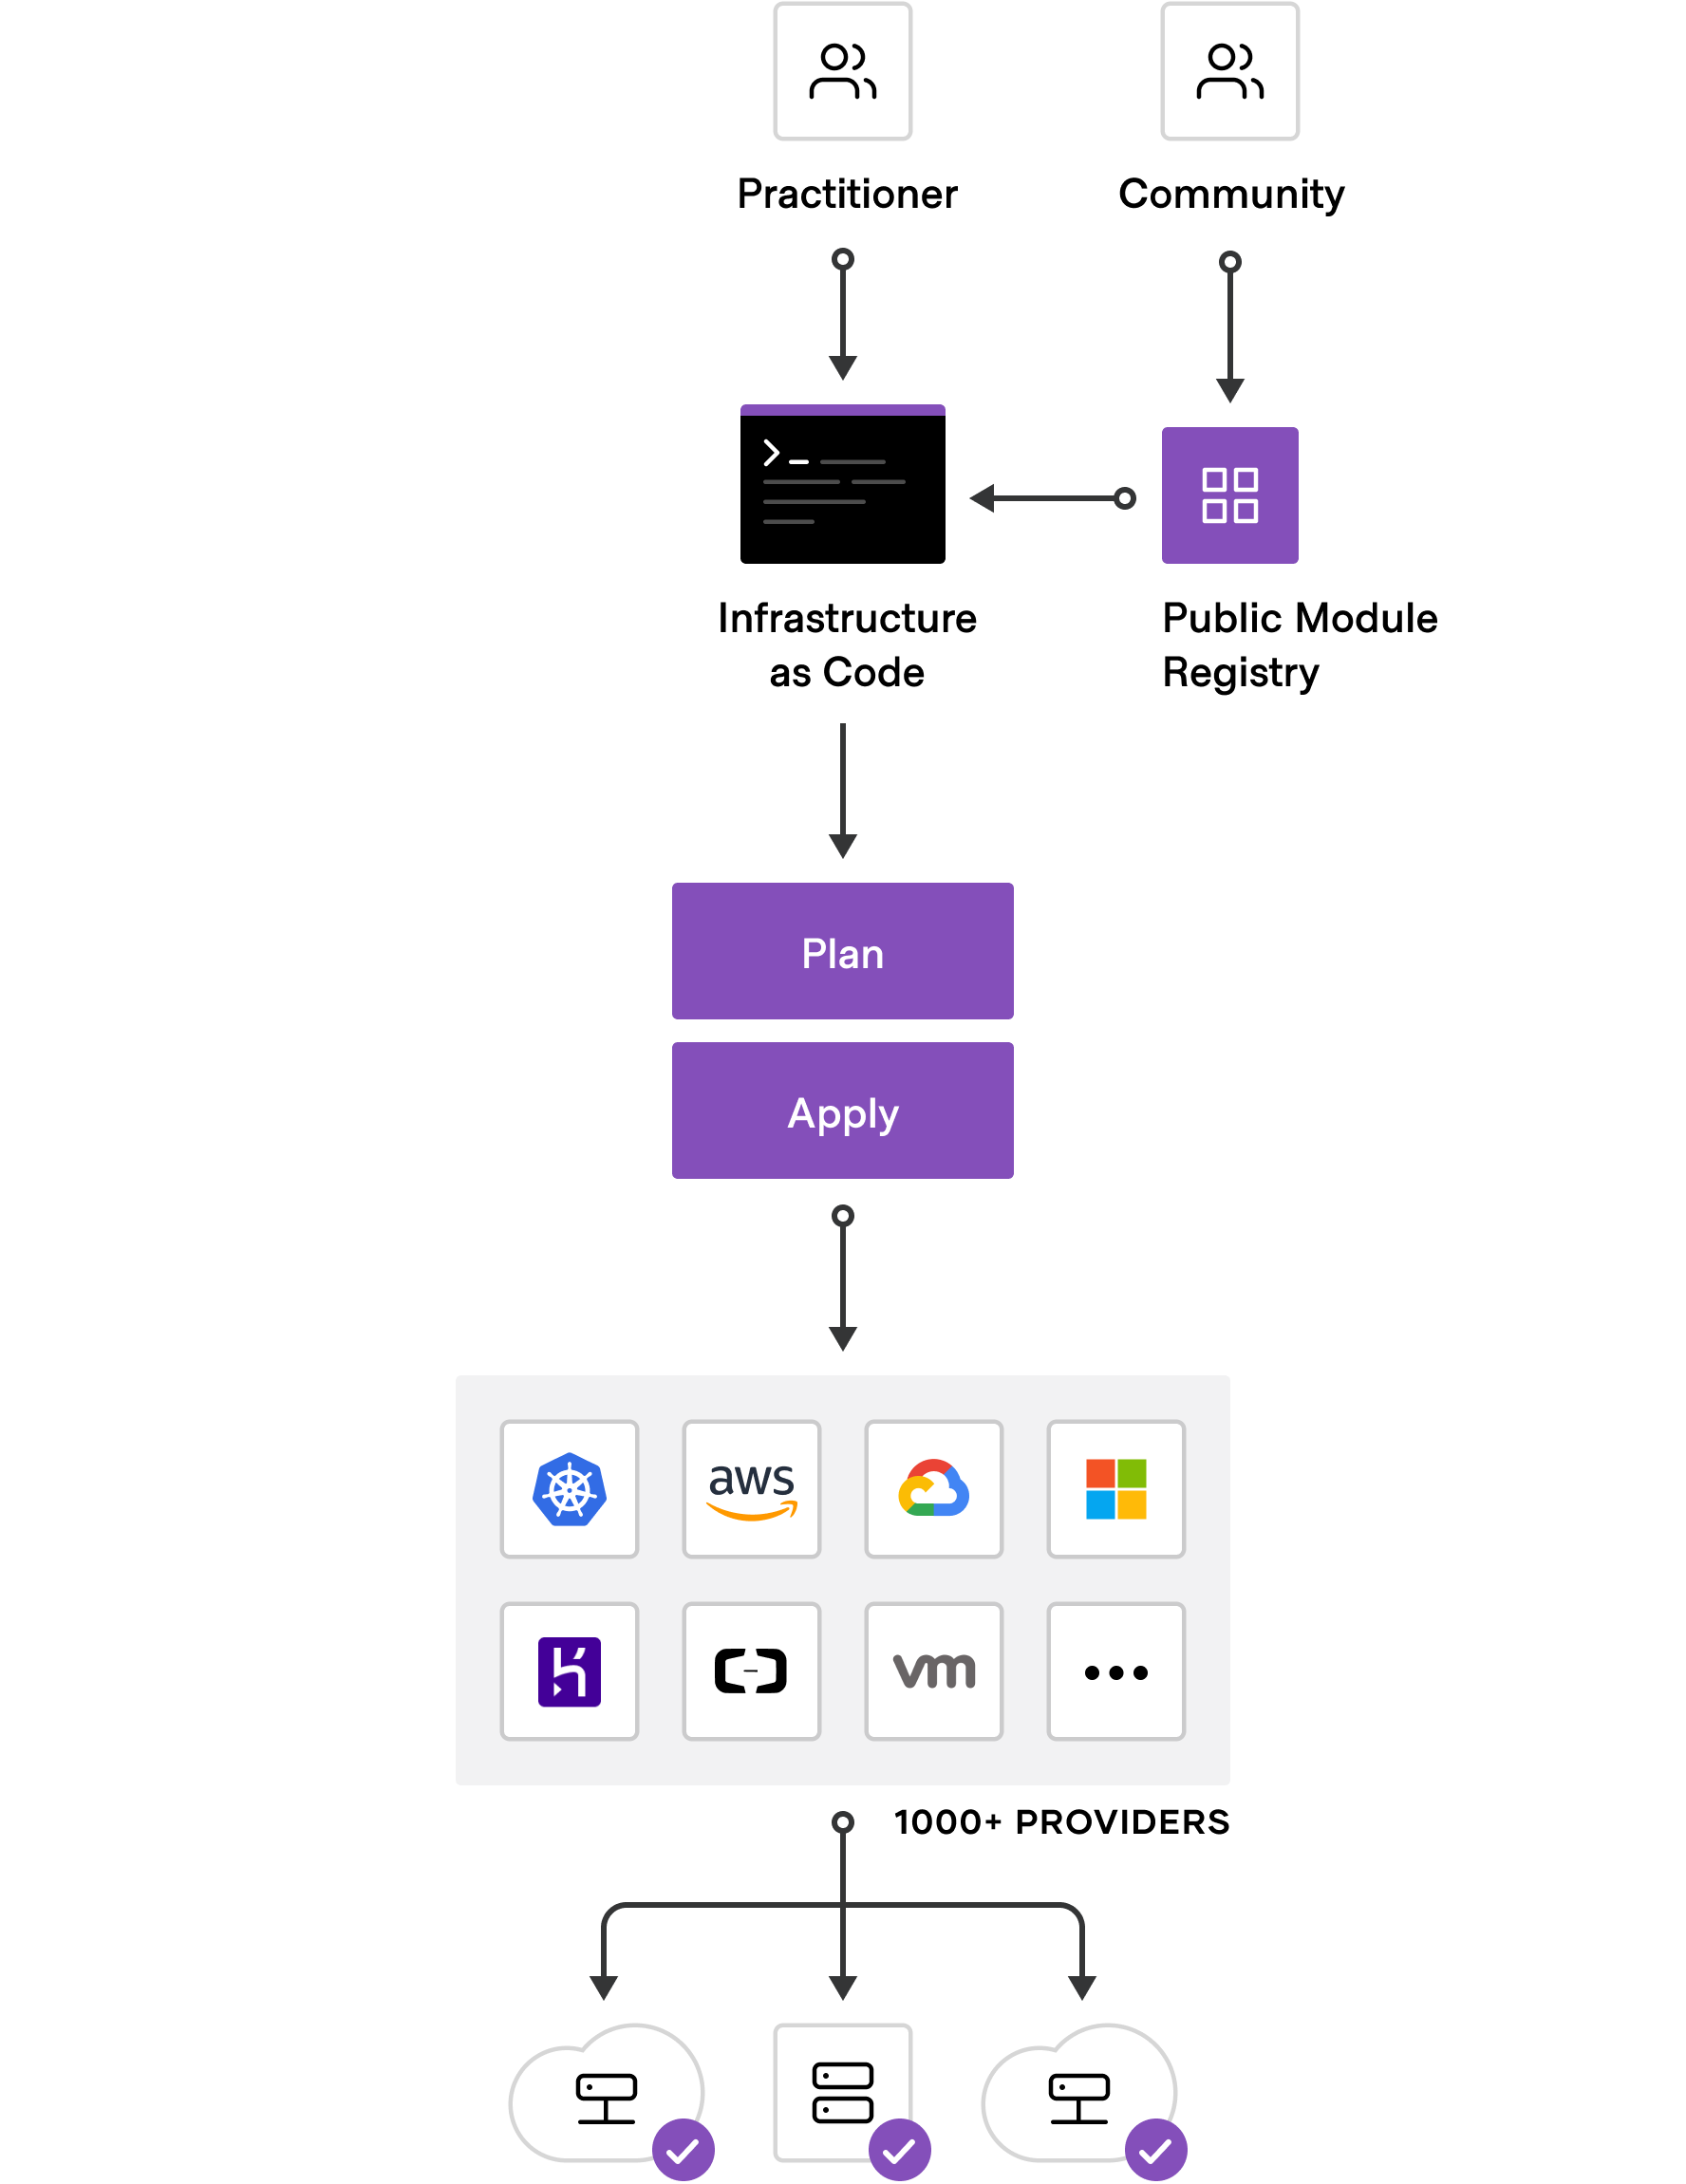
\includegraphics[width=\textwidth,keepaspectratio]{./assets/writeplanapply.png}
    \end{column}
\end{columns}

\end{frame}

% ....

\begin{frame}{Shall we Demo?}

\begin{center}
I don't use AWS so none of this made sense.
\end{center}

\end{frame}

% ....

\begin{frame}{Shall we Demo?}

\begin{center}
    
\includegraphics[width=140px,keepaspectratio]{./assets/dominos.png}
    Remember, Terraform works with APIs not just cloud providers.
\end{center}

\end{frame}

% ....

\begin{frame}[fragile]{Plan}

\begin{center}
    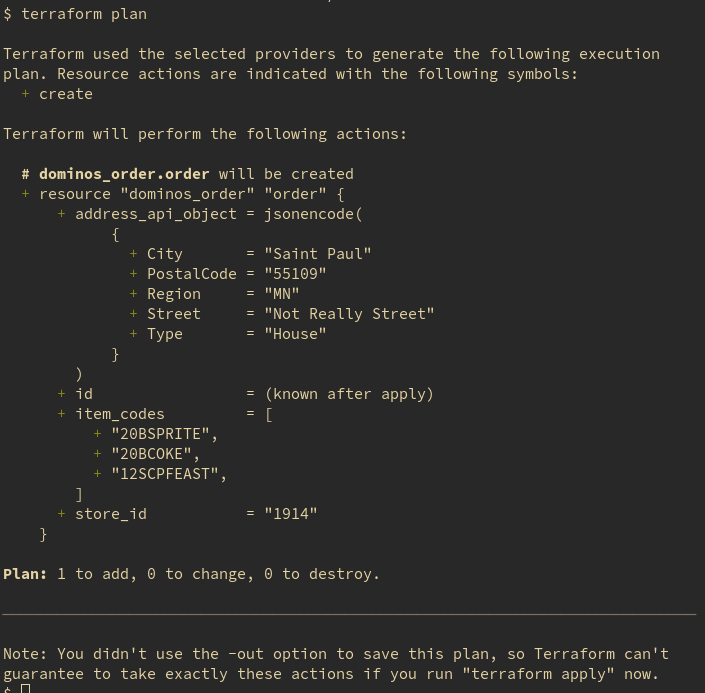
\includegraphics[width=220px,keepaspectratio]{./assets/plan.png}
\end{center}

\end{frame}

% ....

\begin{frame}[fragile]{Demo DNS}

\begin{semiverbatim}
watch -n 0 dig terraform-hello.tolson.io
\end{semiverbatim}

\end{frame}

% ....

\begin{frame}{Launch VMs}

\begin{center}
    Launch some VMs
\end{center}

\end{frame}

% ....

\begin{frame}{Quick action items!}

\begin{itemize}
    \item CICD?
    \begin{itemize}
        \item Terraform is a CLI, wrappers exist but no library.
    \end{itemize}
    \item Launching VMs without Config Management
    \begin{itemize}
        \item Use an image from the cloud provider and tack on cloud-init
        \item Packer!
    \end{itemize}
    \item Modules
    \item Workspaces
    \item Browse the registry
\end{itemize}

\end{frame}

% ....

\begin{frame}{Links and References}

\begin{itemize}
    \item Docs: https://www.terraform.io/docs/language/index.html
    \item Great tutorials: https://learn.hashicorp.com/terraform
    \item Browze providers: https://registry.terraform.io/
\end{itemize}

\end{frame}

\end{document}
